\section{Quality of Results}

As described in~\ref{section:goal_and_scope}, the quality of the generated city is difficult to measure objectively.

% Do models correctly integrate with third-party software such as Blender \cite{blender}?
\textbf{Q1}: \newline
The generated models imports correctly into Blender~\cite{blender}.
Integration with other third-party tools however, would have to be tested more thoroughly as Blender was the main tool used for ensuring exported models could be imported correctly to an external tool. 

Although, the 3D models are imported correctly in terms of the model data there exists some unintended visual differences.
These differences are however, a consequence of the different rendering pipelines between Unity and any other third-party tool.
Figure~\ref{fig:blender_shading_result} showcases these visual differences.

% TODO(anton): Add Figure of resulting model imported into blender
\begin{figure}[h!]
  \centering
  % \includegraphics[width=0.6\textwidth]{figure/blender_shading_result.jpg}
  \caption{Visual differences between the generated Unity model.}
  \label{fig:blender_shading_result}
\end{figure}


% How well is the codebase structured for replacement and expansion of features?
\textbf{Q2}: \newline
As the generation is divided into a number of sub-generators it would be easy to add more generators on to the total generation.
Furthermore, the generators themselves are structured in a way that adding more content to them, or modifying them should be a simple adaptation to make. 

% How much notable variety is there in the generated content?
\textbf{Q3}: \newline
When discussing the variety of the generated cities the group distinguished between the overarching structural variety and the variety in textures and shapes of the content.
In terms of the topological structure or layout of the generated cities the group is content with the variety offered.
Each city has a unique look and vary in their size and layout in a way that the group considers realistic enough.
This variety is showcased in Figure~\ref{fig:discussion_city_layout_variety}.

\begin{figure}[h!]
  \centering
  \begin{subfigure}[b]{0.455\textwidth}
    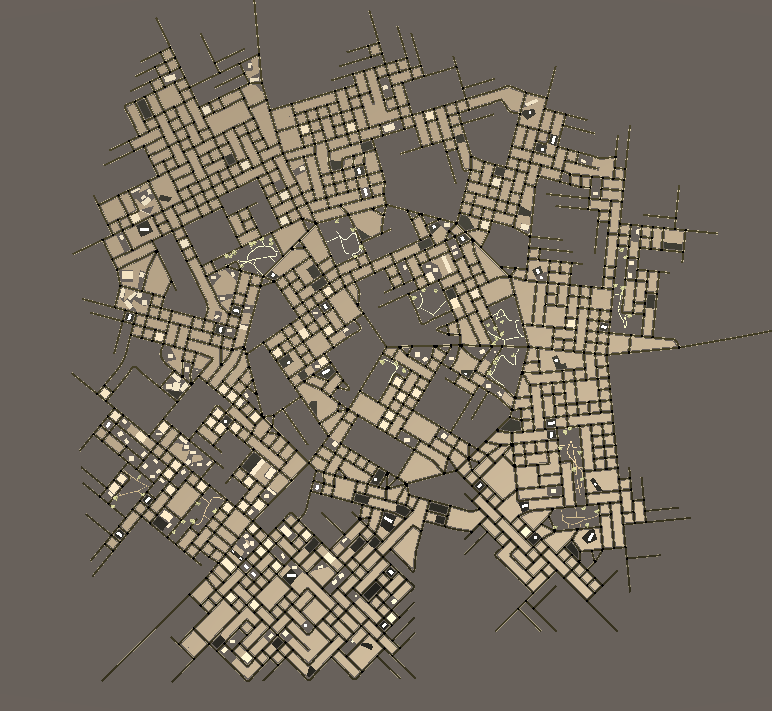
\includegraphics[width=\textwidth]{figure/discussion_city_layout_1}
  \end{subfigure}
  \quad
  \begin{subfigure}[b]{0.45\textwidth}
    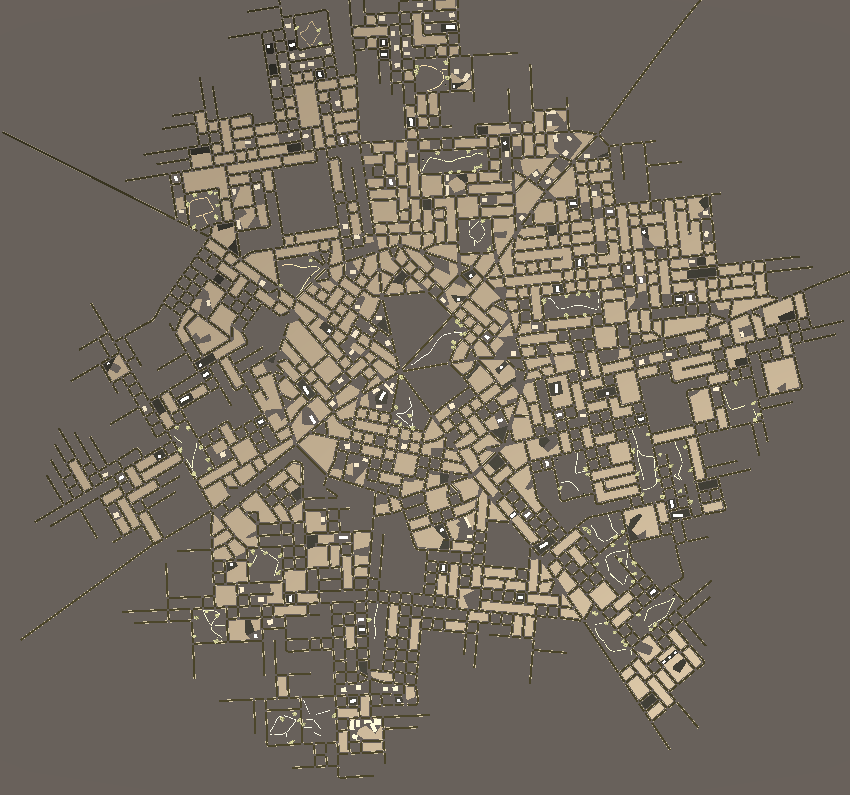
\includegraphics[width=\textwidth]{figure/discussion_city_layout_2}
  \end{subfigure}
  \caption{Cities generated after two consecutive runs under the same conditions highlighting the structural variety.}
  \label{fig:discussion_city_layout_variety}
\end{figure}

The variety in textures and shape variety of skyscrapers, buildings and roads are however limited.
Roads for example, always have the same appearance in terms of their shape and texture.

% How much control do the users have over the generation?
\textbf{Q4}: \newline
% TODO(anton): find other description than seed-based
The degree of control offered to the user is, with a few exceptions, at the level of supplying static settings to each subgenerator.
The exception to this is that the user can dynamically place individual cities and re-generate the content for each subgenerator.
This distinction highlights an important design choice of either creating a city editor with PCG capabilities or a seed-based city generator capable of producing an infinite world with no dynamic user input whatsoever.
CityCraft, tries to be both in the sense that each subgenerator is essentially seed-based but imposes some user choices in the placement of cities for example.
Since the goal was for CityCraft to be a rough tool for generating cities that designers later could refine, the option for allowing the user to edit specific roads or alter the content of a selected block might not be deemed essential but would nevertheless significantly aid a designer and improve the level of control.

Diving into the controls available to the users.
The user has some varying level of control over the generation at different stages of the generation pipeline.
Terrain generation offers the most options available while the city generator offers no parameters to the user. 

Marking the territory on which the user wants to place a city is not entirely accurate when making the marked area very small. 
On the bright side the user has the ability to undo the work of a generator if that has left him unpleased, an area of improvement here would have been to allow the user to mark a territory of the world after generation is done and be able to re-generate that section.
This however was deemed quite time-demanding and will be left as an area of future work. 

% Are the cities suitable for use in digital media such as games and film?
\textbf{Q5}: \newline


% Are users without technical expertise able to correctly use the application?
\textbf{Q6}: \newline
However, the user interface could be improved to provide better feedback to the user.

% Are there any known visual artifacts in the models?
\textbf{Q7}: \newline
% TODO(anton): These are not artifacts as they are intended 
% One visual artifact we are aware of would be that buildings as well as parking lots are generated right on top of the terrain.
% The larger flaw resulting from this would be that it would seem impossible for theoretical cars to reach the generated parking lots, without driving on top of the grass that is.
% Had there been more time, a solution to this would have been implemented by the group but a lot of things were prioritized more heavily and this is therefore also left as an area of future work. 
% two of the approaches that were considered were either filling the entire plots with asphalt (which would probably have looked the best had there been a suiting texture) and would definitely have looked the best for the buildings.
% The other approach that was considered was somehow creating road from the road network to the parking lot, this however was deemed to be very difficult due to the design of the road network. 

% Are there any known bugs or crashes in the application?
\textbf{Q8}: \newline
placement of cities rarely crashes/freezes the program
murar (roads) rare


